\chapter{2023/11/06}\label{20231106}

\section{Real and virtual displacement
实位移和虚位移}\label{real-and-virtual-displacement-ux5b9eux4f4dux79fbux548cux865aux4f4dux79fb}

\emph{见附录B。}

\section{Something about tensors
一些关于张量的讨论}\label{something-about-tensors-ux4e00ux4e9bux5173ux4e8eux5f20ux91cfux7684ux8ba8ux8bba}

\subsection*{(1) Projection tensor
投影张量}\label{projection-tensor-ux6295ux5f71ux5f20ux91cf}

\begin{center}
    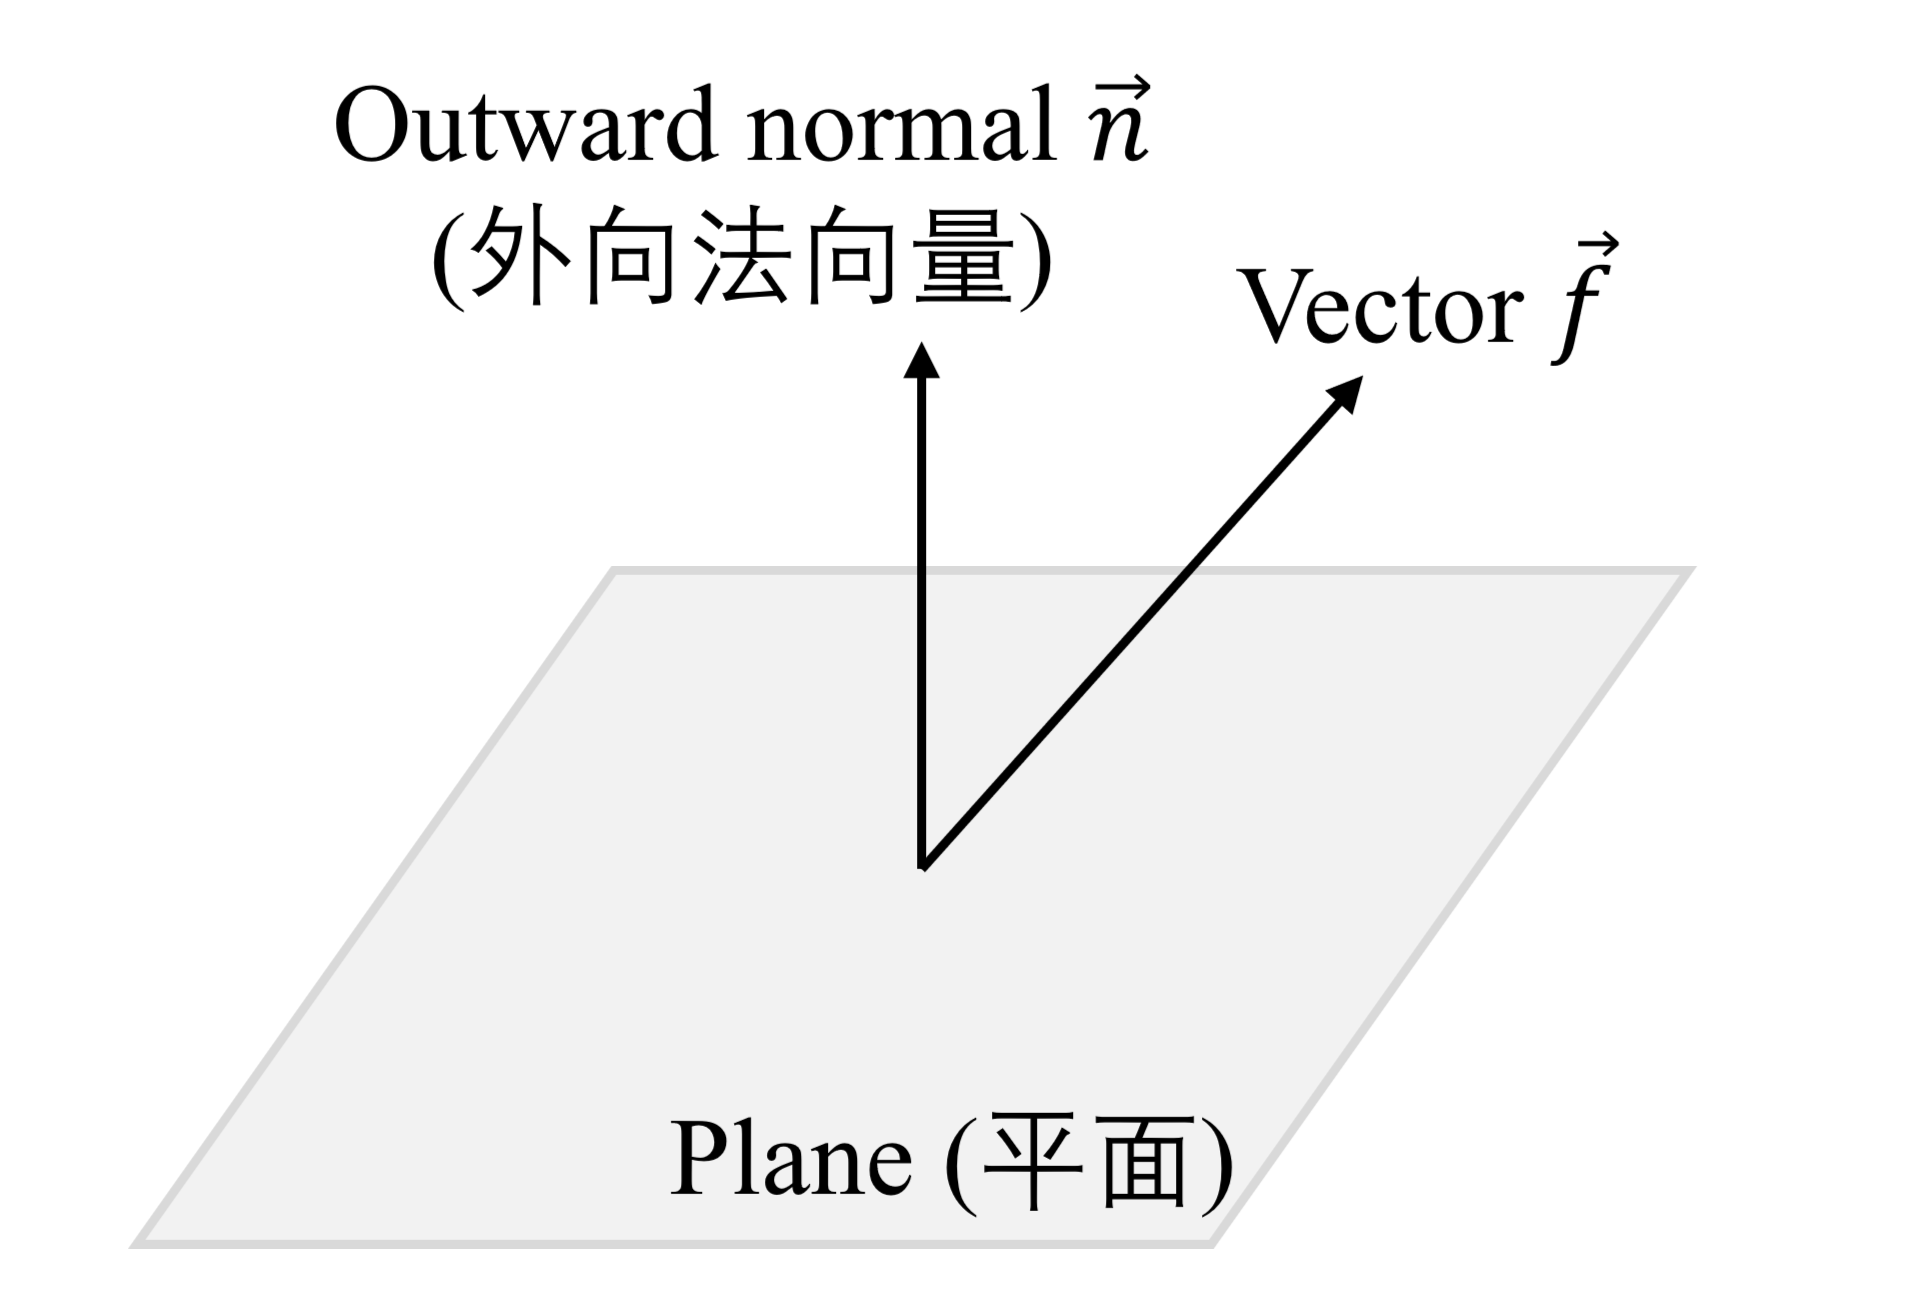
\includegraphics[height=120pt]{assets/Projection_Tensor.png}
    \captionof{figure}{Projection tensor}
\end{center}

Fig 15.1 shows a plain with an outward normal \(\boldsymbol n\)
(\(\boldsymbol n \cdot \boldsymbol n = \boldsymbol n^2 = 1\)), and we
can get the projection of the vector \(\boldsymbol f\):
\[\boldsymbol f_\perp = (\boldsymbol f \cdot \boldsymbol n) \boldsymbol n = \boldsymbol f \cdot (\boldsymbol n \otimes \boldsymbol n). \quad (*)\]

Thus we can get
\[\boldsymbol f_{/\!/} = \boldsymbol f - \boldsymbol f_\perp = \boldsymbol f - \boldsymbol f \cdot (\boldsymbol n \otimes \boldsymbol n) = \boldsymbol f \cdot (\mathbf e - \boldsymbol n \otimes \boldsymbol n).\]

Let \[\mathbf P = \mathbf e - \boldsymbol n \otimes \boldsymbol n,\] and
we call \(\mathbf P\) the \textbf{projection tensor of rank 2
(二阶投影张量)}. An interesting piece of quality of \(\mathbf P\) is:
\begin{align*}
    \mathbf P^2 & = (\mathbf e - \boldsymbol n \otimes \boldsymbol n)^2 \\
    & = \mathbf e^2 - 2 \boldsymbol n \otimes \boldsymbol n + (\boldsymbol n \otimes \boldsymbol n) \cdot (\boldsymbol n \otimes \boldsymbol n) \\
    & = \mathbf e - 2 \boldsymbol n \otimes \boldsymbol n + \boldsymbol n \otimes (\boldsymbol n \cdot \boldsymbol n) \otimes \boldsymbol n \\
    & = \mathbf e - 2 \boldsymbol n \otimes \boldsymbol n + \boldsymbol n \otimes \boldsymbol n\\
    & = \mathbf e - \boldsymbol n \otimes \boldsymbol n \\
    & = \mathbf P.
\end{align*}

Note:

\begin{enumerate}
\def\labelenumi{\arabic{enumi}.}
\tightlist{}
\item Above, \(\otimes\) stands for tensor product (张量积).
\item 
  The proof of \((*)\): \begin{align*}
   \boldsymbol f \cdot (\boldsymbol n \otimes \boldsymbol n) & = (f_k \boldsymbol e_k) \cdot (n_i n_j \boldsymbol e_i \otimes \boldsymbol e_j) \\
   & = (f_k \boldsymbol e_k \cdot n_i n_j \boldsymbol e_i) \boldsymbol e_j \\
   & = f_k n_i n_j \delta_{ik} \boldsymbol e_j \\
   & = f_i n_i n_j \boldsymbol e_j \\
   & = (\boldsymbol f \cdot \boldsymbol n) \boldsymbol n.
  \end{align*}
\end{enumerate}

\subsection*{(2) Moment of inertia tensor 惯性张量
\(\boldsymbol I\)}\label{moment-of-inertia-tensor-ux60efux6027ux5f20ux91cf-boldsymbol-i}

Angular momentum is \begin{align*}
    \boldsymbol L & = \int \boldsymbol r \times \mathrm d \boldsymbol p \\
    & = \int \boldsymbol r \times \rho \boldsymbol v \mathrm dV \\
    & = \rho \int \boldsymbol r_i \times (\boldsymbol \omega \times \boldsymbol r_i) \mathrm dV \\
\end{align*}
\begin{align*}
    & = \rho \int [\boldsymbol \omega (\boldsymbol r_i \cdot \boldsymbol r_i) - \boldsymbol r_i (\boldsymbol r_i \cdot \boldsymbol \omega)] \mathrm dV \\
    & = \rho \int [\boldsymbol \omega r_i^2 - (\boldsymbol r_i \otimes \boldsymbol r_i) \boldsymbol \omega] \mathrm dV \\
    & = \left[ \rho \int (r_i^2 \mathbf e - \boldsymbol r_i \otimes \boldsymbol r_i) \mathrm dV \right] \cdot \boldsymbol \omega.
\end{align*}

From \(\boldsymbol L = \boldsymbol I \cdot \boldsymbol \omega\), we can
see that
\[\boldsymbol I = \rho \int (r_i^2 \mathbf e - \boldsymbol r_i \otimes \boldsymbol r_i) \mathrm dV,\]
which, written in index form, is
\[I_{ij} = \rho \int \left[ (x^2 + y^2 + z^2) \delta_{ij} - x_ix_j \right]\mathrm dV.\]

Written in Cartesian coordinates are: \[\left\{
    \begin{array}{l}
        \displaystyle I_{xx} = \rho \int \left( y^2 + z^2 \right) \mathrm dV, \\
        \displaystyle I_{yy} = \rho \int \left( x^2 + z^2 \right) \mathrm dV, \\
        \displaystyle I_{zz} = \rho \int \left( x^2 + y^2 \right) \mathrm dV, \\
    \end{array}
\right.
\quad \text{and} \quad
\left\{
    \begin{array}{l}
        \displaystyle I_{xy} = \rho \int xy \mathrm dV, \\
        \displaystyle I_{yz} = \rho \int yz \mathrm dV, \\
        \displaystyle I_{xz} = \rho \int xz \mathrm dV. \\
    \end{array}
\right.\]

\section[The conservation of the LRL vector 拉普拉斯--龙格--楞次矢量守恒]{Two methods of deriving the conservation of the Laplace--Runge--Lenz (LRL) vector under a central force field that follows the inverse square law 两种推导平方反比有心力场下拉普拉斯--龙格--楞次矢量守恒的方法}\label{two-methods-of-deriving-the-conservation-of-the-laplacerungelenz-lrl-vector-under-a-central-force-field-that-follows-the-inverse-square-law-ux4e24ux79cdux63a8ux5bfcux5e73ux65b9ux53cdux6bd4ux6709ux5fc3ux529bux573aux4e0bux62c9ux666eux62c9ux65af-ux9f99ux683c-ux695eux6b21ux77e2ux91cfux5b88ux6052ux7684ux65b9ux6cd5}

The Laplace--Runge--Lenz (LRL) vector \(\boldsymbol A\) is
\[\boldsymbol A = \boldsymbol p \times \boldsymbol L - m \kappa \hat {\boldsymbol r}.\]

The following discussion is set under this specific central force field
(有心力场) \(U(r)\): \[U(r) = - {GMm \over r} = - {\kappa \over r}.\]

In this central force field, there are three conserved qualities
(守恒量):

\begin{itemize}
\tightlist{}
\item
  \(\displaystyle E = {p^2 \over 2m} - {\kappa \over r}\)
\item 
  \(\displaystyle \boldsymbol L = \boldsymbol r \times \boldsymbol p\)
\item
  \(\displaystyle \boldsymbol A = \boldsymbol p \times \boldsymbol L - m \kappa \hat {\boldsymbol r}\)
\end{itemize}

\subsection*{(1) Method 1}\label{method-1}

\[\boldsymbol A = \boldsymbol p \times \boldsymbol L - m \kappa \hat {\boldsymbol r}.\]

\[\dfrac{\mathrm d \boldsymbol A}{\mathrm dt} = \dot {\boldsymbol p} \times \boldsymbol L + \boldsymbol p \times \dot {\boldsymbol L} - m \kappa \dfrac{\mathrm d \hat {\boldsymbol r}}{\mathrm dt}.\]

Here, \(\boldsymbol L\) is conserved, and thus
\(\dot {\boldsymbol L} = \boldsymbol 0.\)

According to Newton's laws of motion, we have
\[\dot {\boldsymbol p} = \boldsymbol f = - {\kappa \over r^2} \hat {\boldsymbol r}.\]

Using transport theorem, we know that
\[\dfrac{\mathrm d \hat {\boldsymbol r}}{\mathrm dt} = \left( \dfrac{\mathrm d \hat {\boldsymbol r}}{\mathrm dt} \right)_r + \boldsymbol \omega \times \hat {\boldsymbol r} = \boldsymbol \omega \times \hat {\boldsymbol r}.\]

Thus, \begin{align*}
    \dfrac{\mathrm d \boldsymbol A}{\mathrm dt} & = \left(- {\kappa \over r^2} \hat {\boldsymbol r} \right) \times m r^2 \boldsymbol \omega - m \kappa (\boldsymbol \omega \times \hat {\boldsymbol r}) \\
    & = - m \kappa \hat {\boldsymbol r} \times\boldsymbol \omega - m \kappa \boldsymbol \omega \times \hat {\boldsymbol r} \\
    & = \boldsymbol 0.
\end{align*}

\subsection*{(2) Method 2}\label{method-2}

\begin{align*}
    \dfrac{\mathrm d \boldsymbol A}{\mathrm dt} & = \dot {\boldsymbol p} \times \boldsymbol L + \boldsymbol p \times \dot {\boldsymbol L} - m \kappa \dfrac{\mathrm d \hat {\boldsymbol r}}{\mathrm dt} \\
    & = \left(- {\kappa \over r^2} \hat {\boldsymbol r} \right) \times \left( \boldsymbol r \times m {\mathrm d \boldsymbol r \over \mathrm dt} \right) - m \kappa {1 \over r} {\mathrm d \boldsymbol r \over \mathrm dt} +a {m \kappa \over r^2} \boldsymbol r {\mathrm dr \over \mathrm dt} \\
    & = - {m \kappa \over r^3} \left[ \boldsymbol r \times \left( \boldsymbol r \times {\mathrm d \boldsymbol r \over \mathrm dt} \right) + r^2 {\mathrm d \boldsymbol r \over \mathrm dt} - \boldsymbol r r {\mathrm d r \over \mathrm dt} \right]\\
    & = - {m \kappa \over r^3}\left[ \boldsymbol r \left( \boldsymbol r \cdot {\mathrm d \boldsymbol r \over \mathrm dt} \right) - r^2 {\mathrm d \boldsymbol r \over \mathrm dt} + r^2 {\mathrm d \boldsymbol r \over \mathrm dt} - \boldsymbol r r {\mathrm d r \over \mathrm dt} \right]\\
    & = \boldsymbol 0.
\end{align*}
